\section{Millisecond Pulsars in Globular Clusters}
\label{sec:cases}

Due to the high stellar densities found within globular clusters, dynamical interactions between stars take place in these systems much more frequently than they do among stars in the Galactic Plane. As a result, large numbers of low-mass X-ray binaries (LMXBs) and millisecond pulsars (MSPs) are each found within globular clusters. At present, a total of 340 MSPs have been identified within 45 different Milky Way globular clusters (see \url{https://www3.mpifr-bonn.mpg.de/staff/pfreire/GCpsr.html}, and Refs.~\cite{Manchester:2004bp,Fermi-LAT:2023zzt}). The majority of these pulsars have only been observed at radio wavelengths, as they are too distant to be detected by Fermi. In fact, Fermi's Third Pulsar Catalog~\cite{Fermi-LAT:2023zzt} contains only four MSPs that are located within a globular cluster: 
%
PSR J1717+4308A in NGC 6341, PSR J1823-3021A in NGC 6624, J1824-2452A in NGC 6626, and PSR J1835-3259B in NGC 6652. 

The number of MSPs within a given globular cluster is correlated with that cluster's overall visible-band luminosity, $L_V$ (a proxy for stellar mass), and stellar encounter rate, $\Gamma_e$. 

\noindent
The stellar encounter rate within a globular cluster is given by~\cite{2003ASPC..296..245V,1987IAUS..125..187V}
%
\begin{align}
\Gamma_e = \frac{4\pi}{\sigma_c} \int \rho^2(r) r^2 dr,
\end{align}
%
where $\rho(r)$ is the stellar density profile of the cluster and $\sigma_c$ is the velocity dispersion near its core. Throughout this analysis, we make use of the stellar encounter rates tabulated in Ref.~\cite{Bahramian:2013ihw} (and as we list in Table~\ref{tab:tab7-9-hopper-linden}).

In this study, we will consider the following five hypotheses for estimating the number of MSPs that will, on average, be found within a given globular cluster:
%
\begin{enumerate}
    \item {A case in which the mean number of MSPs in a globular cluster is proportional to its stellar encounter rate, $\langle N_{\rm MSP} \rangle = R_{\rm MSP} \, \Gamma_e$. This approximate scaling might be expected if MSPs in globular clusters are formed largely through stellar interactions.}
    \item{A case in which the relationship between the stellar encounter rate and the expected number of pulsars within a globular cluster is not linear, but instead scales as $\langle N_{\rm MSP} \rangle = R_{\rm MSP} \, \Gamma_e^{0.7}$. Empirically speaking, this hypothesis is preferred over that of a strictly linearly proportional relationship~\cite{deMenezes:2018ilq,Feng:2023htd}.}
    \item{A case in which the mean number of MSPs in a globular cluster is proportional to its visible luminosity, $\langle N_{\rm MSP} \rangle = R_{\rm MSP}\, L_V$.}
    \item{A case in which the mean number of MSPs in a globular cluster is related to a combination of its stellar encounter rate and visible luminosity, $\langle N_{\rm MSP} \rangle = R_{\rm MSP} \, \Gamma_e+ R'_{\rm MSP} \, L_V$.}
    \item{A case in which the mean number of MSPs in a globular cluster is related to a combination of a non-linear scaling to its stellar encounter rate and its visible luminosity, $\langle N_{\rm MSP} \rangle = R_{\rm MSP} \, \Gamma_e^{0.7}+ R'_{\rm MSP} \, L_V$.}
\end{enumerate}
%
For further discussion regarding the dynamics of globular clusters and empirical relationships between their observed parameters, see Refs.~\cite{Feng:2023htd,Ye:2022yxt,deMenezes:2018ilq,Fragione:2018jxd}.

\begin{figure}[t]
\centering
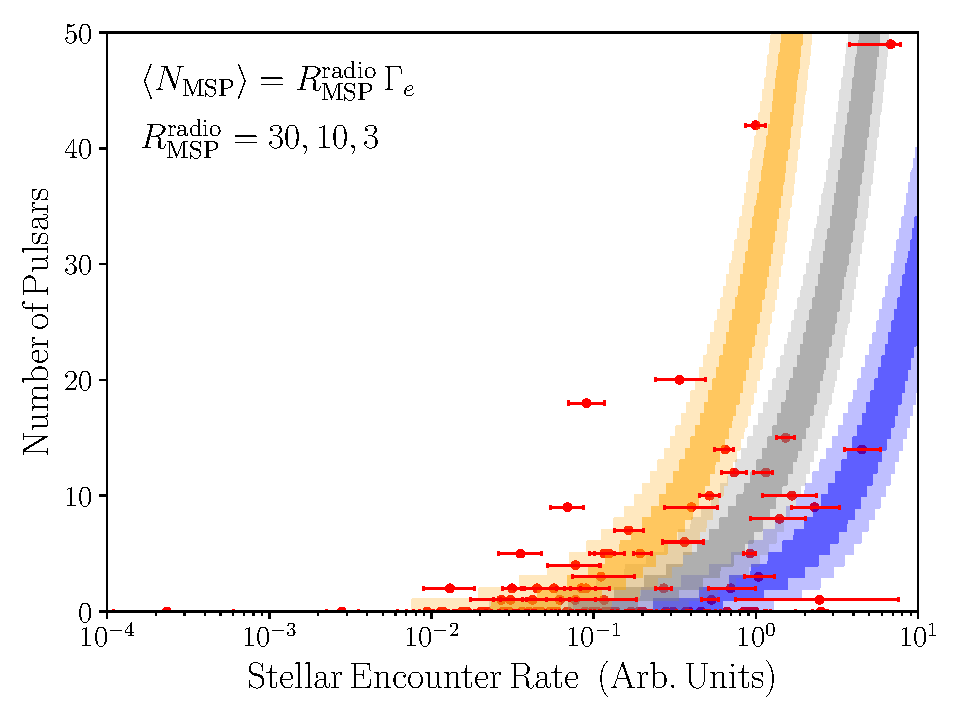
\includegraphics[width=0.49\textwidth]{img/radio-dataplot.pdf}
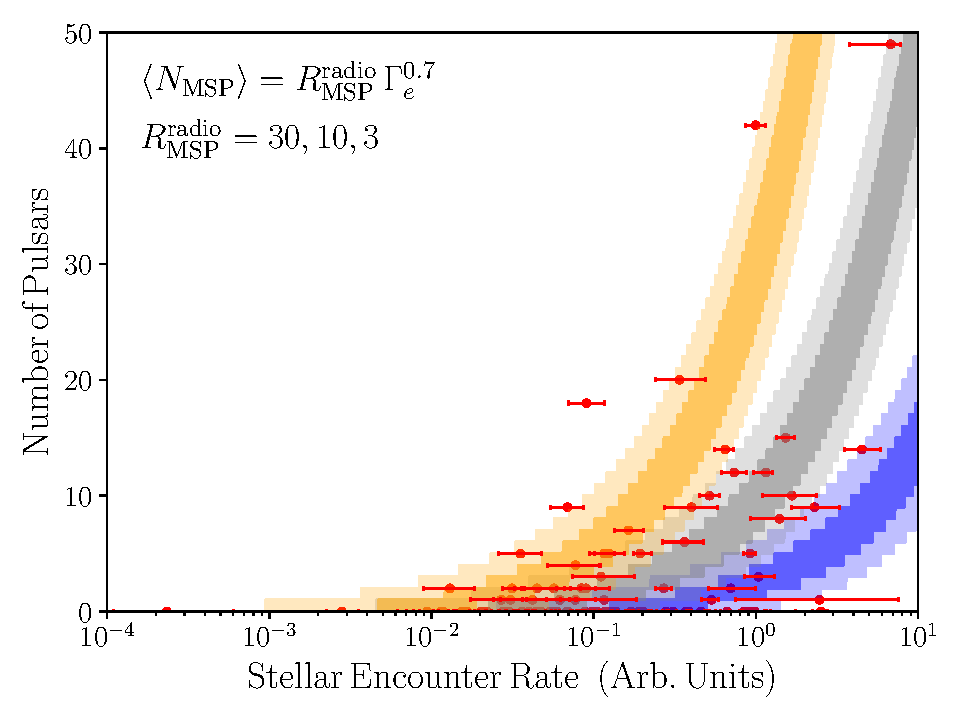
\includegraphics[width=0.49\textwidth]{img/radio-case2-dataplot.pdf}
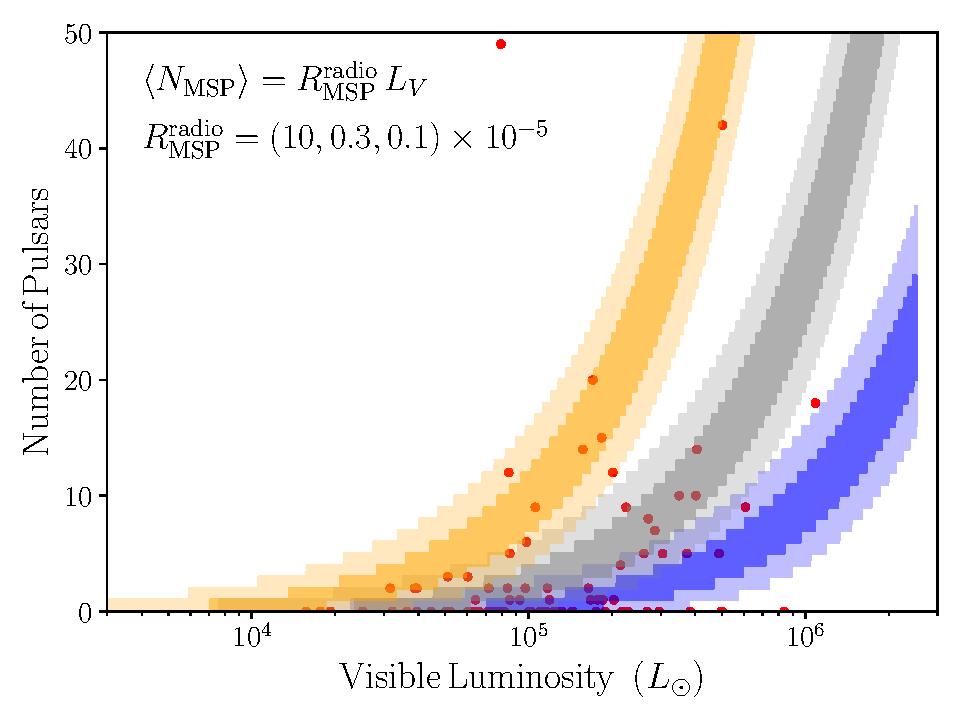
\includegraphics[width=0.49\textwidth]{img/radio-case3-dataplot.pdf}
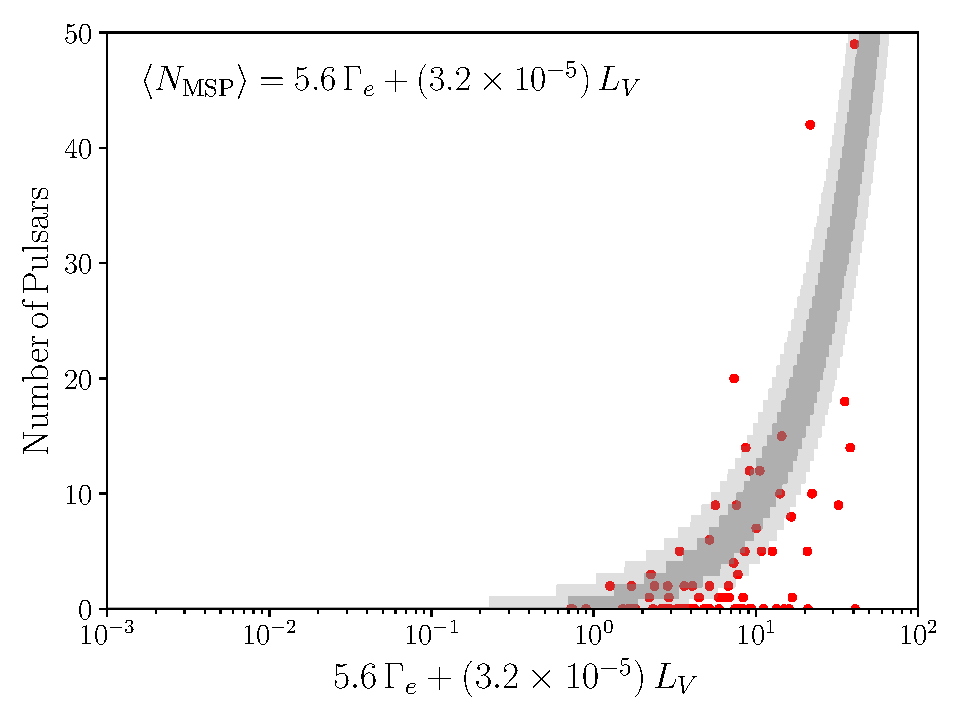
\includegraphics[width=0.49\textwidth]{img/radio-case4-dataplot.pdf}
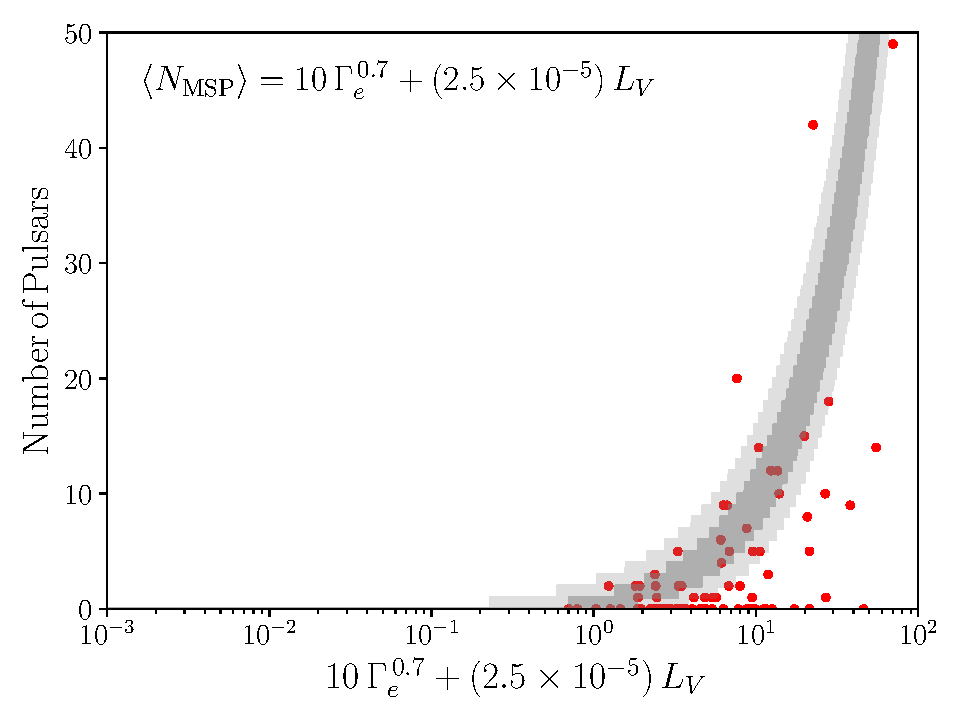
\includegraphics[width=0.49\textwidth]{img/radio-case5-dataplot.pdf}
\caption{The number of known millisecond pulsars in each of the 87 globular clusters considered in this study (those with $L_V > 10^5 \, L_{\odot}$ or $\Gamma_e > 0.01$) as a function of combinations of the stellar encounter rate, $\Gamma_e$, and visible luminosity, $L_V$ (in units of solar luminosities). Also shown are colored bands representing the predicted number of MSPs (68.27\% and 95.45\% containment) in each case, for selected values of $R_{\rm MSP}^{\rm Radio}$. The stellar encounter rate is normalized such that $\Gamma_e =1$ for NGC 104.}
\label{fig:radio}
\end{figure}

Throughout the remainder of this study, we will focus on the 87 globular clusters that have either $L_V > 10^5 \, L_{\odot}$ or $\Gamma_e > 0.01$ (in units such that $\Gamma_e =1$ for the case of NGC 104). In Fig.~\ref{fig:radio}, we plot the number of MSPs that are known to exist in each of these 87 globular clusters, as a function of their stellar encounter rate, visible luminosity, or combinations of these parameters. We also show bands which represent the predicted relationships between these quantities, for selected values of $R_{\rm MSP}^{\rm Radio}$.\footnote{While we take $R_{\rm MSP}$ and $R'_{\rm MSP}$ to be related to the predicted number of gamma-ray MSPs in a given globular cluster, the same quantities with the superscript ``Radio'' correspond to the predicted number of radio MSPs. Due to the different beaming angles of pulsars in the gamma-ray and radio bands, these quantities are not necessarily the same.} 
The inner (outer) bands are calculated such that they cover 68.27\% (95.45\%) of a Poisson distribution for a mean value of $\langle N_{\rm MSP}^{\rm Radio} \rangle$. Even by eye, it is clear that the correlation is less tight for the case of $\langle N_{\rm MSP} \rangle = R_{\rm MSP}\,{\Gamma_e}$ than for $\langle N_{\rm MSP} \rangle = R_{\rm MSP}\,{\Gamma_e}^{0.7}$, or for $\langle N_{\rm MSP} \rangle = L_V$. The tightest correlations are found for combinations of $\Gamma_e$ and $L_V$ (as shown in the final two frames). One should bear in mind that the current catalog of the MSPs in globular clusters is incomplete, limiting the utility of any quantitative comparisons. That being said, the results presented in Fig.~\ref{fig:radio} provide us with motivation to consider the five hypotheses described above for the anticipated number of MSPs in globular clusters.

